\documentclass{beamer}

\usepackage{amsmath}

\usetheme{AnnArbor}
\usecolortheme{crane}
\usefonttheme[onlymath]{serif}

\title{Deep Learning - Foundations and Concepts}
\subtitle{Chapter 17. Generative Adversarial Networks}
\author{nonlineark@github}
\date{\today}

\begin{document}

\begin{frame}
    \titlepage
\end{frame}

\begin{frame}
    \frametitle{Outline}
    \tableofcontents
\end{frame}

\section{Adversarial Training}

\begin{frame}
    \frametitle{Adversarial training}
    Consider a generative model based on a nonlinear transformation from a latent space $z$ to a data space $x$:
    \begin{align*}
        p(z)&=\mathcal{N}(z;0,I) \\
        x&=g(z;w)
    \end{align*}
    However, we cannot determine $w$ by optimizing the likelihood function because this cannot, in general, be evaluated in closed form.
\end{frame}

\begin{frame}
    \frametitle{Adversarial training}
    The key idea of generative adversarial networks, or GANs, is to introduce a second discriminator network, which is trained jointly with the generator network and which provides a training signal to update the weights of the generator.
    \begin{figure}
        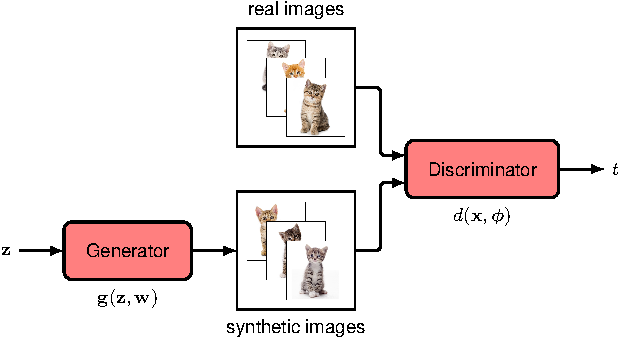
\includegraphics[height=0.5\textheight]{Figure_1.pdf}
    \end{figure}
\end{frame}

\begin{frame}
    \frametitle{Adversarial training}
    \begin{itemize}
        \item The goal of the discriminator network is to distinguish between real examples and synthetic examples, and it is trained by minimizing a conventional classification error function.
        \item Conversely, the goal of the generator network is to maximize this error by synthesizing examples from the same distribution as the training set.
    \end{itemize}
\end{frame}

\begin{frame}
    \frametitle{Loss function}
    We define a binary target variable:
    \begin{equation*}
        t=\begin{cases}
            1,&\textrm{real data,} \\
            0,&\textrm{synthetic data.}
        \end{cases}
    \end{equation*}
    We train the discriminator network using the standard cross-entropy error function:
    \begin{equation*}
        E(w,\phi)=-\frac{1}{N}\sum_{n=1}^{N}(t_{n}\log{}d_{n}+(1-t_{n})\log(1-d_{n}))
    \end{equation*}
    where $d_{n}=d(x_{n};\phi)$. We can write the error function in the form:
    \begin{align*}
        E_{\textrm{GAN}}(w,\phi)=&-\frac{1}{N_{\textrm{real}}}\sum_{n\in\textrm{real}}\log{}d(x_{n};\phi) \\
        &-\frac{1}{N_{\textrm{synth}}}\sum_{n\in\textrm{synth}}\log(1-d(g(z_{n};w);\phi))
    \end{align*}
\end{frame}

\begin{frame}
    \frametitle{Loss function}
    The unusual aspect is the adversarial training whereby the error is minimized with respect to $\phi$ but maximized with respect to $w$:
    \begin{align*}
        \Delta\phi&=-\lambda\nabla_{\phi}E_{n}(w,\phi) \\
        \Delta{}w&=\lambda\nabla_{w}E_{n}(w,\phi)
    \end{align*}
    where $E_{n}(w,\phi)$ denotes the error defined for a mini-batch of data points.
\end{frame}

\begin{frame}
    \frametitle{Loss function}
    The training process:
    \begin{enumerate}
        \item Calculate error for a mini-batch and update $w$.
        \item Generate a new set of synthetic samples.
        \item Calculate error for a mini-batch and update $\phi$.
        \item Generate a new set of synthetic samples.
        \item Go to step 1.
    \end{enumerate}
    If the generator succeeds in finding a perfect solution, then the discriminator network will be unable to tell the difference between the real and synthetic data and hence will always produce an output of $0.5$.
\end{frame}

\begin{frame}
    \frametitle{GAN training in practice}
    \begin{figure}
        \caption{Learning proceeds slowly for the optimal discriminator function $d(x)$}
        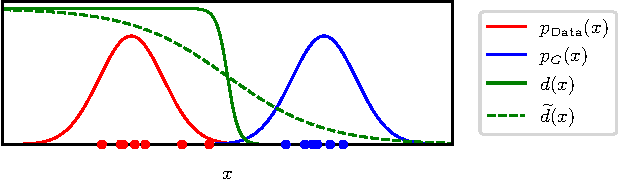
\includegraphics{Figure_2.pdf}
    \end{figure}
\end{frame}

\begin{frame}
    \frametitle{GAN training in practice}
    This can be addressed by using a smoothed version $\tilde{d}(x)$ of the discriminator function:
    \begin{itemize}
        \item The least-squares GAN modifies the discriminator to produce a real-valued output and replaces the cross-entropy error function with a sum-of-squares error function.
        \item The instance noise technique adds Gaussian noise to both the real data and the synthetic samples.
    \end{itemize}
\end{frame}

\begin{frame}
    \frametitle{GAN training in practice}
    For faster training, one change that is often used is to replace the generative network term in the original error function:
    \begin{equation*}
        -\frac{1}{N_{\textrm{synth}}}\sum_{n\in\textrm{synth}}\log(1-d(g(z_{n};w);\phi))
    \end{equation*}
    with the modified form:
    \begin{equation*}
        \frac{1}{N_{\textrm{synth}}}\sum_{n\in\textrm{synth}}\log{}d(g(z_{n};w);\phi)
    \end{equation*}
    \begin{figure}
        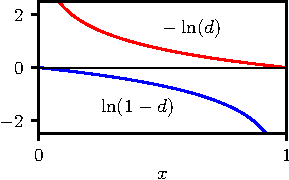
\includegraphics{Figure_3.pdf}
    \end{figure}
\end{frame}

\begin{frame}
    \frametitle{GAN training in practice}
    A more direct way to ensure that the generator distribution $p_{\textrm{G}}(x)$ moves towards the data distribution $p_{\textrm{Data}}(x)$ is to measure how far apart the two distributions are using the Wasserstein distance:
    \begin{itemize}
        \item Wasserstein GAN.
        \item Gradient penalty Wasserstein GAN.
    \end{itemize}
    \href{https://lilianweng.github.io/posts/2017-08-20-gan/}{Further references}.
\end{frame}

\section{Image GANs}

\begin{frame}
    \frametitle{CycleGAN}
    \begin{figure}
        \caption{Examples of image translation using a CycleGAN}
        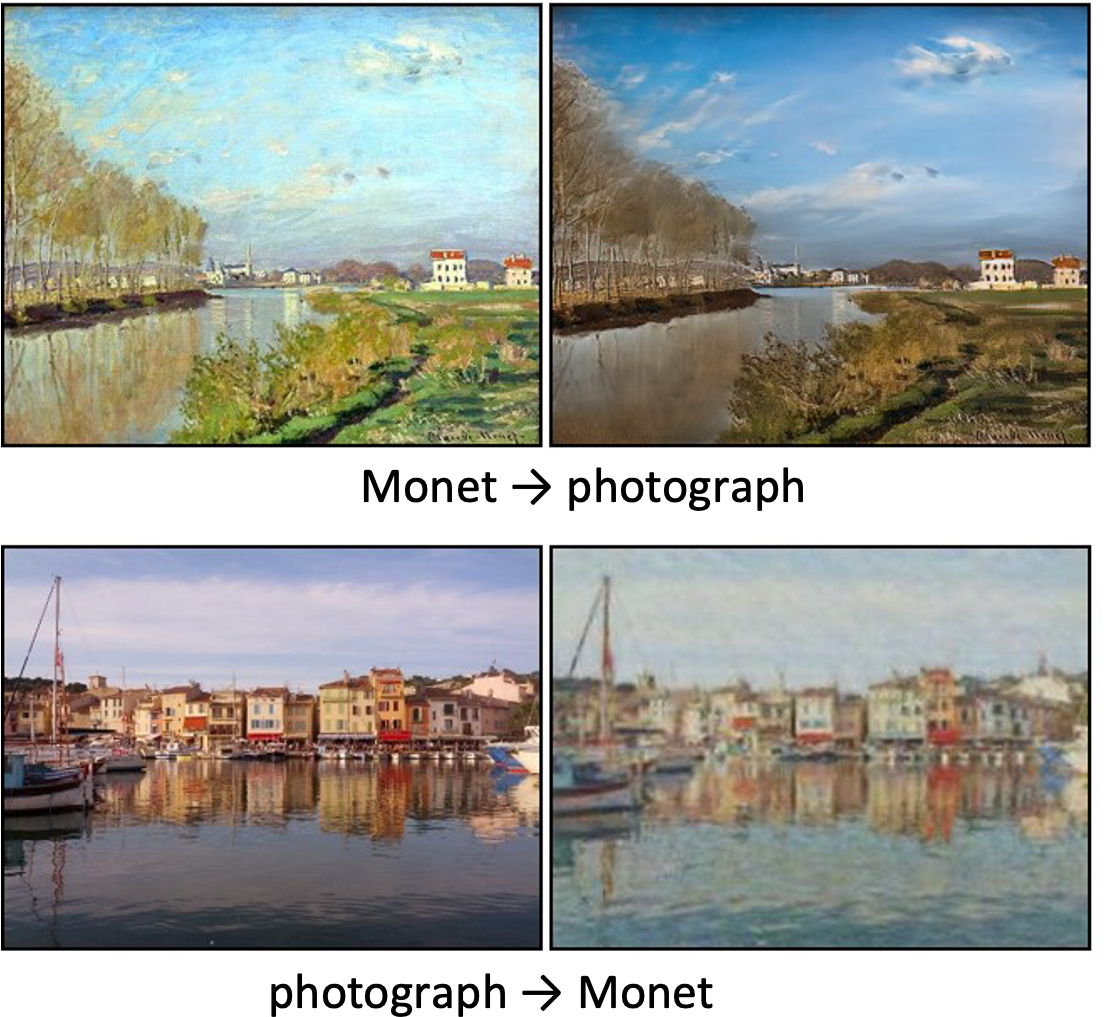
\includegraphics[height=0.7\textheight]{Figure_6.png}
    \end{figure}
\end{frame}

\begin{frame}
    \frametitle{CycleGAN}
    The aim is to learn two bijective mappings, one that goes from the domain $X$ of photographs to the domain $Y$ of Monet paintings and one in the reverse direction:
    \begin{itemize}
        \item The generator $g_{X}(y;w_{X})$ takes as input a sample painting $y\in{}Y$ and generates a corresponding synthetic photograph.
        \item The discriminator $d_{X}(x;\phi_{X})$ distinguishes between synthetic and real photographs.
        \item The generator $g_{Y}(x;w_{Y})$ takes as input a sample photograph $x\in{}X$ and generates a corresponding synthetic painting.
        \item The discriminator $d_{Y}(y;\phi_{Y})$ distinguishes between synthetic and real paintings.
    \end{itemize}
\end{frame}

\begin{frame}
    \frametitle{CycleGAN}
    To ensure that the generated painting looks like the photograph and vice versa, we introduce an additional term in the loss function called the cycle consistency error:
    \begin{align*}
        E_{\textrm{cyc}}(w_{X},w_{Y})&=\frac{1}{N_{X}}\sum_{n\in{}X}||g_{X}(g_{Y}(x_{n}))-x_{n}||_{1} \\
        &+\frac{1}{N_{Y}}\sum_{n\in{}Y}||g_{Y}(g_{X}(y_{n}))-y_{n}||_{1}
    \end{align*}
    where $||\cdot||_{1}$ denotes the L1 norm. The total error function is given by:
    \begin{equation*}
        E_{\textrm{GAN}}(w_{X},\phi_{X})+E_{\textrm{GAN}}(w_{Y},\phi_{Y})+\eta{}E_{\textrm{cyc}}(w_{X},w_{Y})
    \end{equation*}
    where the coefficient $\eta$ determines the relative importance of the GAN errors and the cycle consistency error.
\end{frame}

\begin{frame}
    \frametitle{Representation learning}
    GANs can also be used for representation learning in which rich statistical structure in a data set is revealed through unsupervised learning. The latent space has become organized in ways that are semantically meaningful.
\end{frame}

\begin{frame}
    \frametitle{Representation learning}
    \begin{figure}
        \caption{Taking smooth walks through latent space between randomly generated locations}
        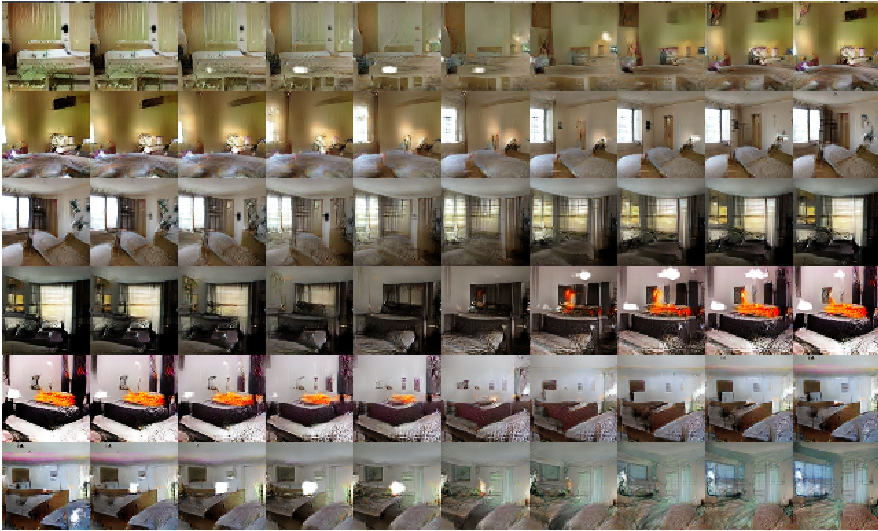
\includegraphics[height=0.6\textheight]{Figure_9.pdf}
    \end{figure}
\end{frame}

\begin{frame}
    \frametitle{Representation learning}
    \begin{figure}
        \caption{An example of vector arithmetic in the latent space of a trained GAN}
        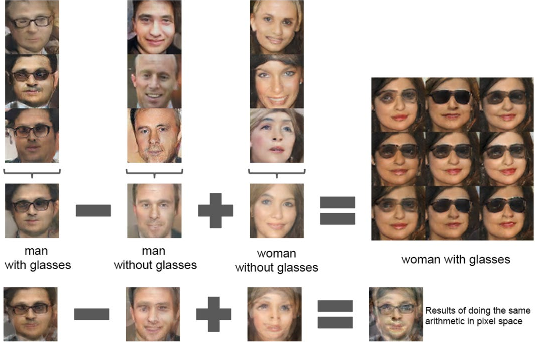
\includegraphics{Figure_10.pdf}
    \end{figure}
\end{frame}

\end{document}